\section{Discussion of the Results}
\label{section:discussion}

\begin{figure}[t]
\begin{center}
\subfigure{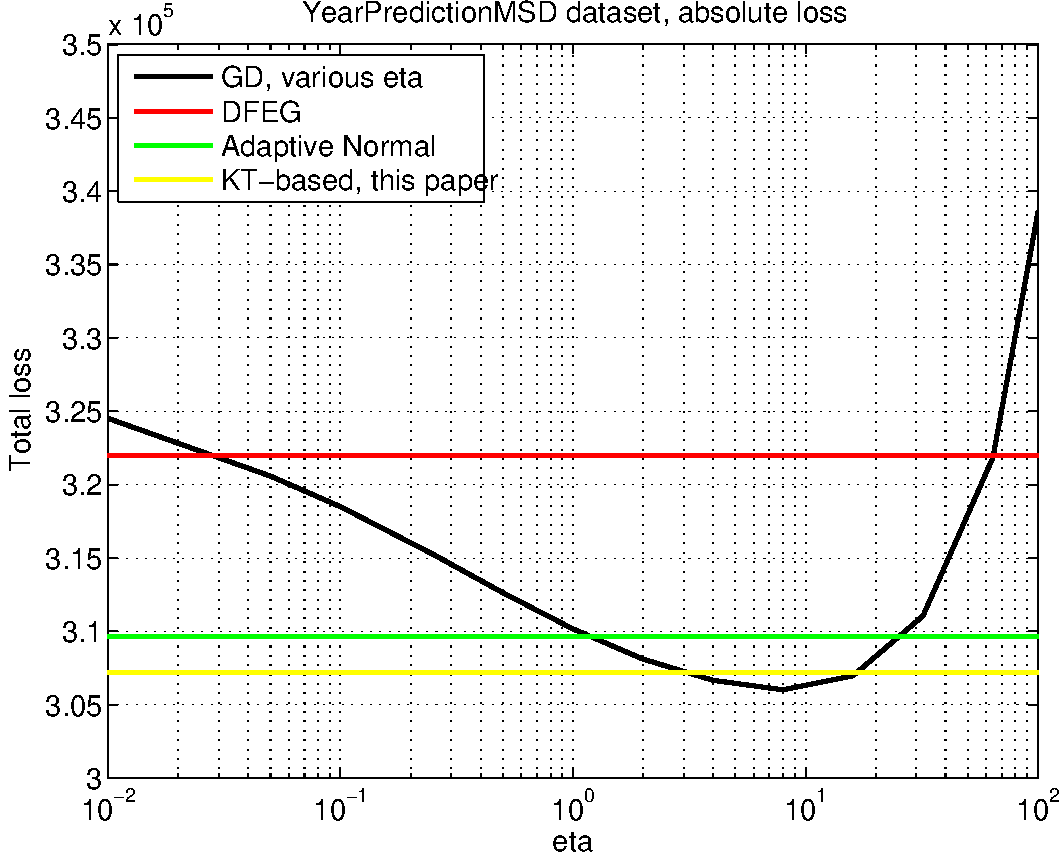
\includegraphics[width=0.32\textwidth]{figs/yearpredictionmsd_kt-crop.pdf}}
\subfigure{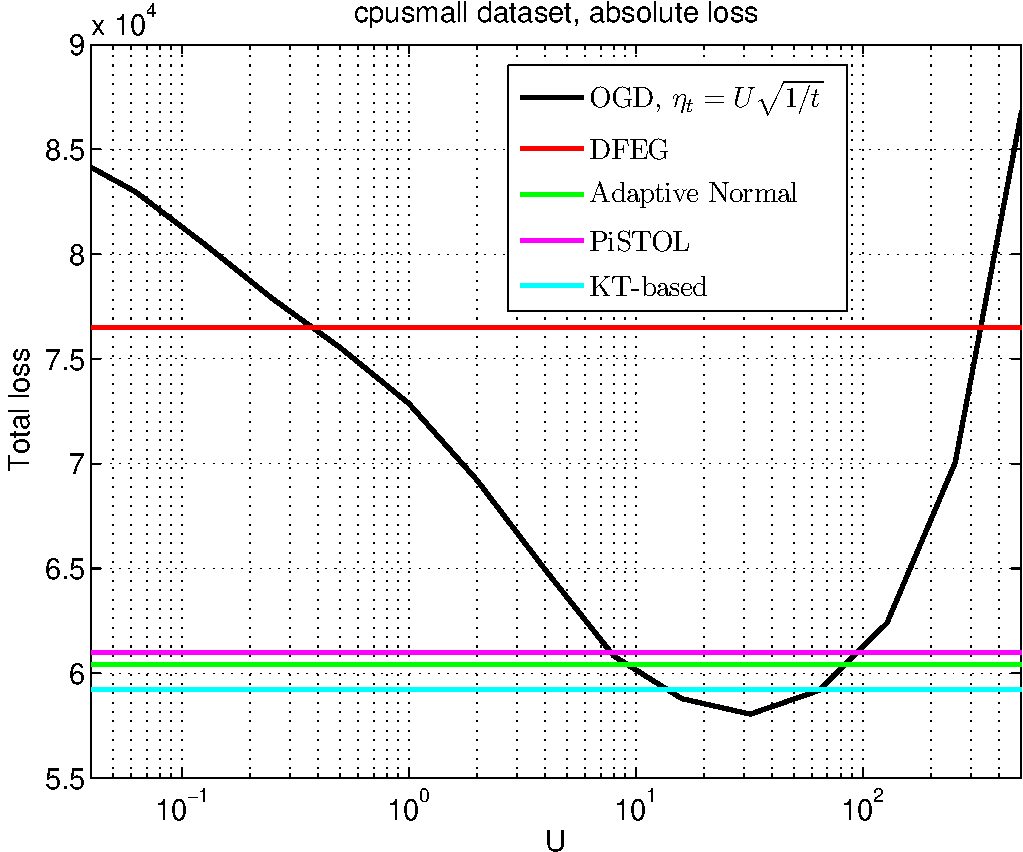
\includegraphics[width=0.32\textwidth]{figs/cpusmall_kt-crop.pdf}}
\subfigure{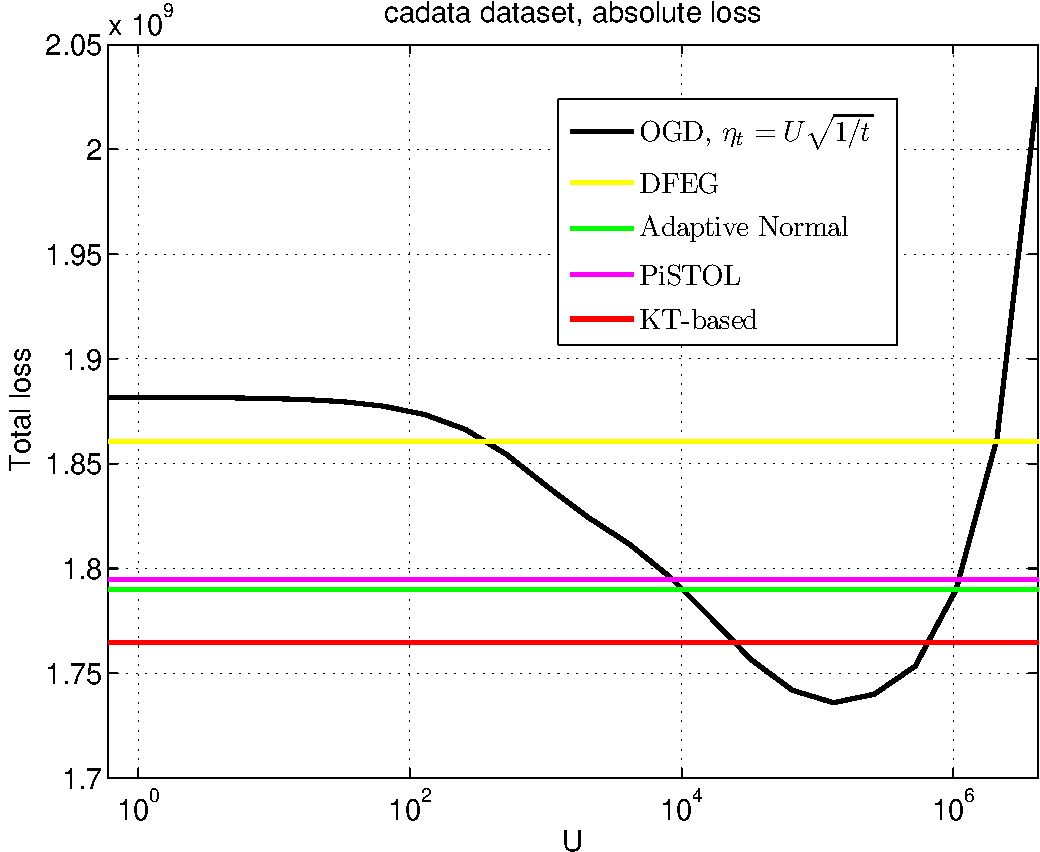
\includegraphics[width=0.32\textwidth]{figs/cadata_kt-crop.pdf}}
\caption{\footnotesize{Total loss versus parameter of \ac{OGD}, compared with parameter-free algorithms DFEG~\cite{Orabona-2013}, Adaptive Normal~\cite{McMahan-Orabona-2014}, PiSTOL~\cite{Orabona-2014} and Algorithm~\ref{algorithm:kt-hilbert-space-olo}.}}
\label{fig:exp_olo}
\end{center}
\end{figure}

\begin{figure}[t]
\begin{center}
\subfigure{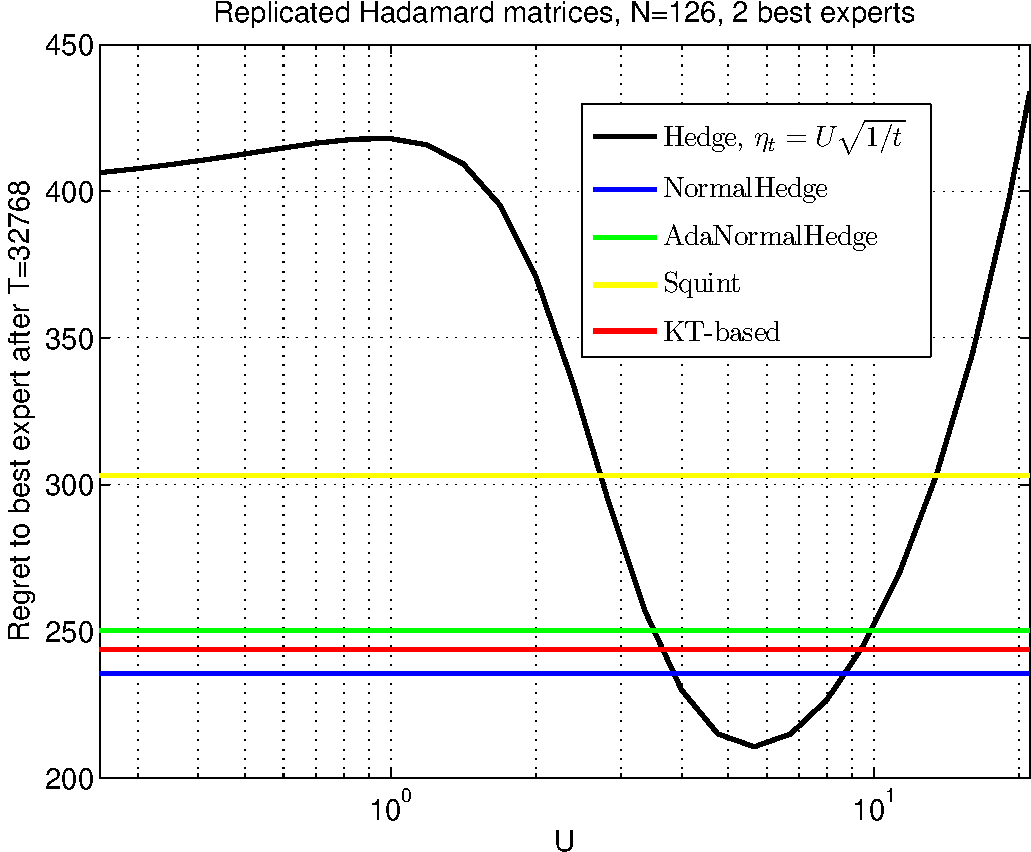
\includegraphics[width=0.32\textwidth]{figs/fig1-crop.pdf}}
\subfigure{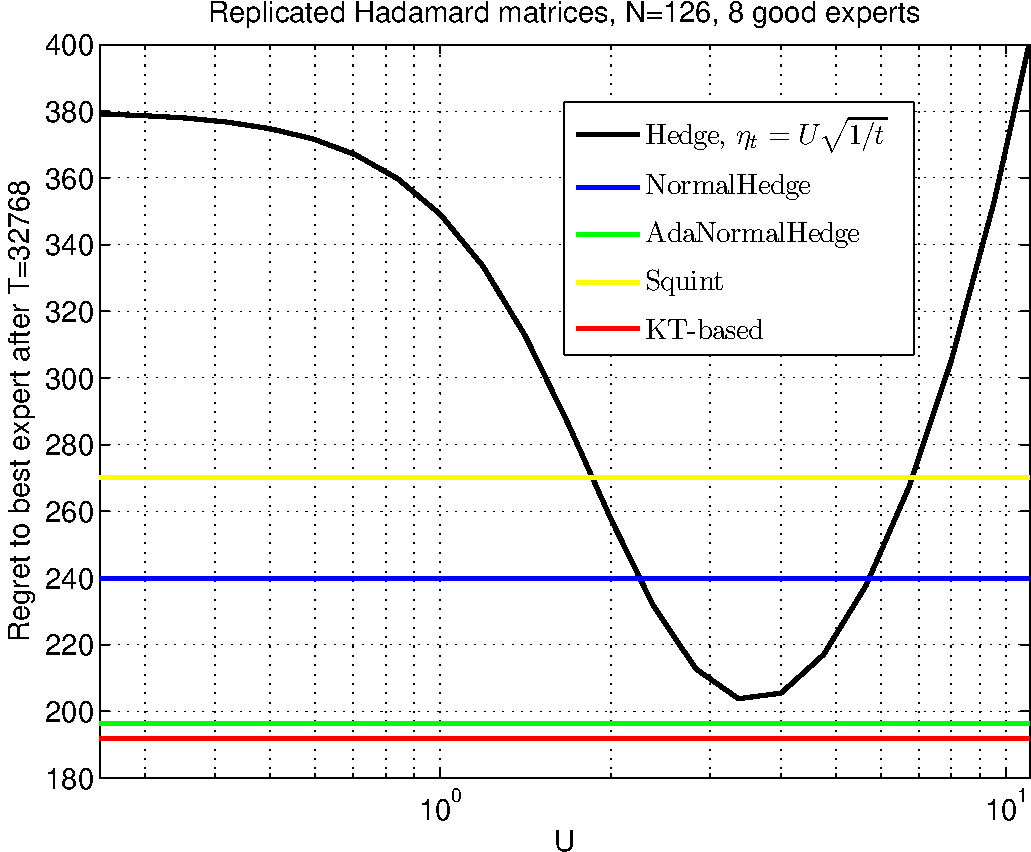
\includegraphics[width=0.32\textwidth]{figs/fig2-crop.pdf}}
\subfigure{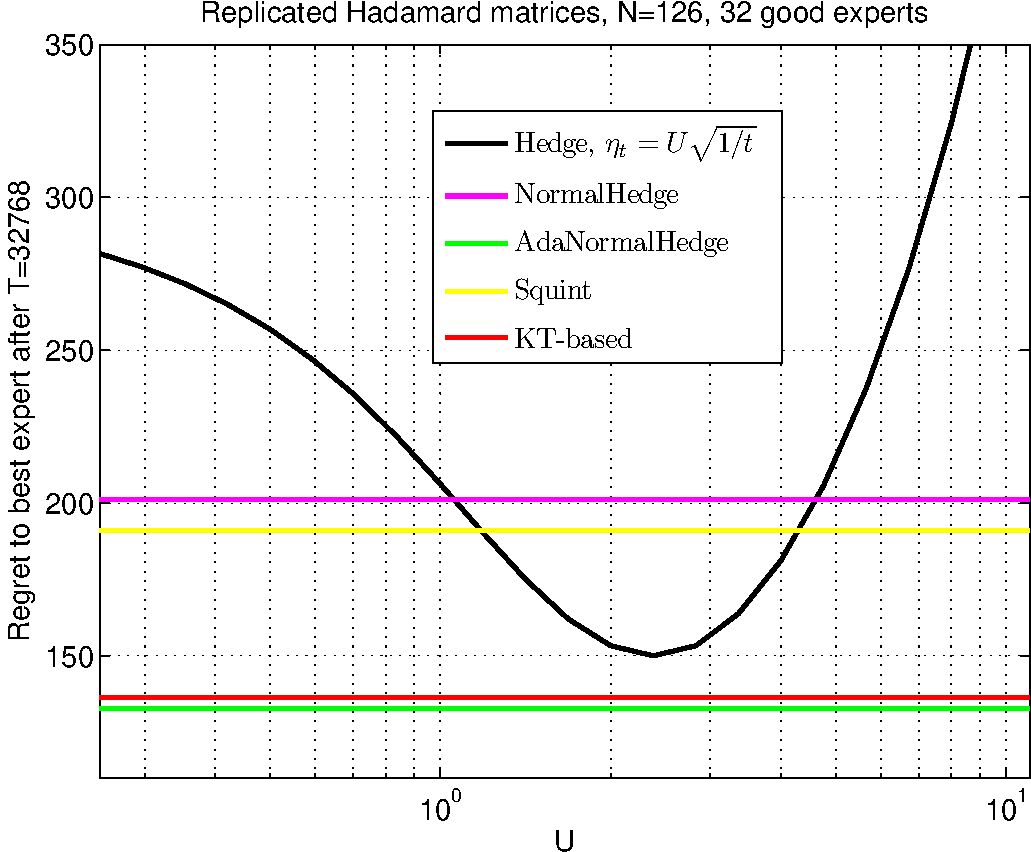
\includegraphics[width=0.32\textwidth]{figs/fig3-crop.pdf}}
\caption{\footnotesize{Regrets to the best action after $T = 32768$ rounds, versus learning rate of Hedge. The best actions are defined as $\epsilon=0.025$ better than the others. The competitor algorithms are NormalHedge~\cite{Chaudhuri-Freund-Hsu-2009}, AdaNormalHedge~\cite{Luo-Schapire-2015}, Squint~\cite{Koolen-van-Erven-2015}, and Algorithms~\ref{algorithm:kt-experts}.}}
\label{fig:exp_lea}
\end{center}
\end{figure}

We have also run an empirical evaluation mainly to show the difference between
classic online learning algorithms and the parameter-free ones. In
Figure~\ref{fig:exp_olo}, we have used three regression
datasets\footnote{Available at
\url{https://www.csie.ntu.edu.tw/~cjlin/libsvmtools/datasets/}.}, and solved
the \ac{OCO} problem through \ac{OLO}. In all the three cases, we have used the
absolute loss and normalized the input vectors to have L2 norm equal to 1. The
results clearly show that parameter-free algorithms have performance very close
to the \emph{unknown} optimal tuning of the learning rate.

For the setting of \ac{LEA}, we have used the synthetic setting
in~\cite{Chaudhuri-Freund-Hsu-2009}. The dataset is composed by Hadamard
matrices of size 64, where the row with constant values is removed, $k$ rows
are decreasing by $0.025$ and the matrix is replicated in order to generate
$T=32768$ samples. For more details, see~\cite{Chaudhuri-Freund-Hsu-2009}.
Here, the KT-based algorithm is the one in
Algorithm~\ref{algorithm:kt-experts}, where the term $T/2$ is removed, so that
the final regret bound has an additional $\ln T$ term.  Again, we see that the
parameter-free algorithms have a performance close or even better than Hedge
with an oracle tuning of the learning rate.

The interpretation of parameter-free algorithms as coin-betting algorithms is
new. This interpretation, far from being just a mathematical gimmick, reveals
the common hidden structure of previous parameter-free algorithms. For example,
we show that the characteristic of parameter-freeness is just a consequence of
having an algorithm that guarantees the maximum reward possible.  In this
sense, most of the online learning algorithms requiring parameter tuning are
just guaranteeing a suboptimal wealth growth. The concept of ``learning rate''
becomes questionable in the light of the presented results.  At the same time,
the previous ad-hoc choices of the potentials were just approximations of the
optimal obtainable wealth.

In particular, in previous \ac{LEA} papers the potential used for an expert at
time $t$ is $\exp \left(\tfrac{([x]_+)^2}{t} \right)$; see
\citep{Chaudhuri-Freund-Hsu-2009, Luo-Schapire-2014, Luo-Schapire-2015}. In
view of the presented results, this potential is an approximation of the
optimal wealth achievable. Moreover, that potential and the ones
by~\citet{Chernov-Vovk-2010} and \cite{Koolen-van-Erven-2015} are not even,
which introduces a lot of technical difficulties in the analysis. Instead, our
reduction moves the truncation outside of the potential, see
\eqref{eq:gradients_experts_reduction}, making the analysis straightforward.

In the \ac{OLO} setting, \citet{Streeter-McMahan-2012} used a one-dimensional
potential of the form $\exp \left(\tfrac{|x|}{\sqrt{t}}\right)$, the same base
potential as in \ac{EG}~\citep{Kivinen-Warmuth-1997} and
Hedge~\cite{Freund-Schapire-1997}, obtaining a suboptimal regret bound. Notice
that the same suboptimality is present in \ac{EG} and Hedge: the learning rate
has to be tuned with the knowledge of the number of experts.
\citet{Orabona-2013} extended the potential to the infinite dimensional case,
unveiling the connection of the work of \citet{Streeter-McMahan-2012} with
\ac{EG}, but still obtaining a suboptimal bound. The optimal bound has been
obtained in \citet{McMahan-Orabona-2014} with potential of the right form $\exp
\left(\frac{x^2}{t}\right)$ that, as said before, is an excellent coin betting
potential.

% The obtained bounds, in Corollaries~\ref{corollary:kt-hilbert-space-olo-regret}
% and~\ref{corollary:kt-experts-regret}, improve the previous ones and/or
% correspond to simpler algorithms.  In particular, the only known bound for
% \ac{LEA} without a $\ln(\ln(T))$ is due to \citet{Chernov-Vovk-2010} for a
% prediction strategy that does not have a closed form.  Moreover, the reductions
% make possible to transfer any advancement on the problem of coin-betting to
% \ac{OLO} and \ac{LEA}. Notice that since the adaptive Kelly strategy based on
% \ac{KT} estimator is very close to optimal, the only possible improvement is to
% have a data-dependent bound, for example like the ones
% in~\cite{Koolen-van-Erven-2015}.  Indeed, it is very easy to extend the proof
% of our reductions to hold in the data-dependent case as well. For example, it
% is an easy exercise to show that a potential of the form $\exp
% \left(\frac{x^2}{1+\sum_{i=1}^{t-1} \norm{g_{i}}}\right)$ is an excellent coin
% betting potential. Through our reductions, such potential would recover at the
% same time the bounds in \citet{Luo-Schapire-2015} and \citet{Orabona-2014}. It
% is an open problem to design a coin betting potential of the form $\exp
% \left(\frac{x^2}{1+\sum_{i=1}^{t-1} \norm{g_{i}}^2}\right)$, that would allow
% to recover immediately the bounds in~\citet{Koolen-van-Erven-2015} and the
% optimistic bounds for smooth losses in
% \ac{OCO}~\citep{Srebro-Sridharan-Tewari-2010} with a parameter-free algorithm
% (see the discussion in \citet{Orabona-2014}).

% Moreover, as already proved in previous papers, the existence of parameter-free
% algorithms have broad consequences, beyond online learning. For example,
% \citet{Luo-Schapire-2015} prove that a parameter-free expert algorithm can be
% used to design an efficient algorithm that predicts as the best pruning tree.
% In the context of risk minimization over Lipschitz convex losses in an infinite
% dimensional Hilbert space, \citet{Orabona-2014} proved that the parameter-free
% \ac{OLO} can be used to obtain risk bound guarantees that compete with the
% regularized \acl{ERM} solution with oracle tuning of the regularizer. In
% simpler words, the parameter-free
% Algorithm~\ref{algorithm:kt-hilbert-space-olo} can be used to obtain, for
% example, the same risk guarantee of a kernel \acl{SVM} with optimal (unknown)
% tuning of the regularizer.

Regarding the tightness of the reductions, it is easy to see that they are in a
certain sense optimal. In fact, the obtained
Algorithms~\ref{algorithm:kt-hilbert-space-olo} and~\ref{algorithm:kt-experts}
achieves the optimal worst case upper bound on regret, see \cite{Streeter-McMahan-2012,Orabona-2013}
and \cite{Cesa-Bianchi-Lugosi-2006} respectively.
% Also, the reduction in Section~\ref{section:reduction-experts}
% implies a connection between the lower bounds for \ac{OLO} and \ac{LEA}: it is easy to derive an
% $\Omega(\norm{u} \sqrt{T\log(1+\norm{u})})$ lower bound for \ac{OLO} over
% 1-d Hilbert space from the well known $\Omega(\sqrt{T \log N})$
% lower bound for \ac{LEA}.

